\documentclass[conference]{IEEEtran}
\IEEEoverridecommandlockouts

\usepackage{cite}
\usepackage{amsmath,amssymb,amsfonts}
\usepackage{algorithmic}
\usepackage{graphicx}
\usepackage{textcomp}
\usepackage{xcolor}
\usepackage{booktabs}
\usepackage{multirow}
\usepackage{url}
\usepackage{microtype}

\begin{document}

\title{Beyond Contemporary Standard English: A Pilot Study of False-Alarm Fragility in Lightweight Jailbreak Classifiers Under Diachronic and Dialectal Shift}

\author{
    \IEEEauthorblockN{Anjali Ajith, Aishwarya Upadhyay, and Aadya Singh}
    \IEEEauthorblockA{\textit{Department of Computer Science and Engineering} \\
    \textit{Dronacharya College of Engineering, affiliated with Gurugram University}\\
    Gurugram, Haryana, India \\
    Email: \{anjali.ajith, aishwarya.upadhyay, aadya.singh\}@dronacharya.info}
}

\maketitle

\begin{abstract}
Input-filtering classifiers are widely used as perimeter defenses for large language models (LLMs), yet they are usually evaluated on contemporary standard English. We present a controlled pilot study of how lightweight prompt classifiers behave under diachronic (Victorian-register) shift, socio-regional (Indian-English) shift, and their combination, in a $2 \times 2$ factorial design. Using 25 base prompts (15 malicious, 10 benign) taken from published safety benchmarks and rewritten by an LLM under embedding-similarity and length controls, we train four linear classifiers (word TF-IDF and character n-gram features) on the unshifted prompts and evaluate them on the three shifted conditions. Recall on malicious prompts stayed at 1.000 in every condition, whereas the false-positive rate (FPR) on the 10 benign prompts rose from 0 to between 0.2 and 1.0, depending on classifier and condition. With exact paired tests and Holm correction over 12 comparisons, five increases remain significant at $\alpha = 0.05$; the rest are inconclusive at this sample size. AU-ROC stayed at or above 0.973, which suggests that part of the effect reflects a fixed decision threshold rather than lost ranking ability. Exploratory balanced re-weighting suggests that part of the false positives in unweighted models is associated with majority-class prior bias and feature sparsity (substantially for the logistic models, modestly to moderately for LinearSVC and Ridge), but notable residual increases remain, especially in the combined condition. We found no consistent interaction between the two shifts. Because the sample is small and the detectors are simple, we treat the results as hypothesis-generating and outline a larger benchmark and an evaluation of production guardrails.
\end{abstract}

\begin{IEEEkeywords}
Jailbreak detection, prompt classifiers, distribution shift, dialect robustness, false positives, over-refusal, AI safety
\end{IEEEkeywords}

\section{Introduction}
\label{sec:intro}
Production deployments of large language models (LLMs) often combine refusal training with lightweight input classifiers that screen prompts before they reach the model \cite{han2024wildguard, fomin2026whenbenchmarkslie}. Such detectors usually report high accuracy on standard benchmark suites, but those suites are written almost entirely in contemporary standard English, whereas real users write in many registers and dialects.

Prior work has studied how detectors degrade over calendar time as attackers invent new templates \cite{piet2025jailbreaksovertime}, and how safety training fails under translation or past-tense rephrasing \cite{andriushchenko2025refusal, deng2024multilingual}. Dialect-linked false positives are well documented for toxic-language detection \cite{sap2019risk}. To our knowledge, however, the behavior of standalone prompt classifiers under controlled intra-lingual register and dialect shifts, with semantic labels held fixed and benign hard negatives included, has not been studied systematically. We pose the following question: \textit{when the wording of a prompt changes in register or dialect but its meaning and safety label do not, do lightweight classifiers trained on contemporary standard English change their decisions?}

\subsection{Threat Model}
Two risks motivate the question. The first is \textit{evasion}: an attacker rewrites a harmful request in an unfamiliar style to slip past a filter (false negatives). The second is \textit{false-alarm censorship}: a legitimate user writing in a regional dialect or an archaic register is wrongly flagged (false positives). We measure both.

\subsection{Contributions}
\begin{enumerate}
    \item A $2 \times 2$ factorial evaluation design that crosses a temporal axis (contemporary vs. Victorian register) with a regional axis (standard vs. Indian English), keeping safety labels fixed.
    \item A pilot evaluation of four lightweight classifiers on 25 base prompts per condition, reported with exact paired tests, Holm correction, and confidence intervals.
    \item Evidence, at pilot scale, that false positives on benign prompts increase under shift while malicious recall remains 1.000, accompanied by exploratory analyses suggesting that unweighted false alarms are partly associated with class-prior imbalance and feature sparsity, though residual increases persist under combined shift.
\end{enumerate}

\section{Related Work}
\label{sec:related}

\textbf{Temporal shift.} Piet et al. \cite{piet2025jailbreaksovertime} documented how jailbreak detectors degrade over a 10-month period as new attack templates appear. Andriushchenko and Flammarion \cite{andriushchenko2025refusal} showed that past-tense reformulations circumvent refusal training in frontier LLMs. We study a different dimension, the register of historical English prose, applied to benign as well as malicious prompts.

\textbf{Multilingual and cultural safety.} Deng et al. \cite{deng2024multilingual} showed that translating harmful prompts into low-resource languages weakens safety alignment. Later benchmarks extend this to ten country--language pairs \cite{choi2026xlsafetybench}, South Asian languages \cite{pattnayak2026indicjr}, African languages \cite{akinode2026tukabench}, and persuasive jailbreaks in Indian languages \cite{mondal2026indicsafeeval}. These works evaluate generative LLM refusal across languages; we instead isolate variation within English and evaluate dedicated input classifiers.

\textbf{Dialect bias and exaggerated safety.} Sap et al. \cite{sap2019risk} found that dialect markers correlate with toxicity labels and that models trained on such data flag dialectal text more often. XSTest \cite{rottger2024xstest} showed that safety-tuned models refuse benign prompts that resemble unsafe ones. Fomin \cite{fomin2026whenbenchmarkslie} showed that prompt-attack classifiers can learn dataset-identity shortcuts that fail under leave-one-dataset-out testing. Our study combines these concerns for prompt classifiers under dialect and register shift.

\section{Experimental Design}
\label{sec:design}

\subsection{Factorial Transformation Space}
We define a transformation $T(x, \tau, \rho)$ of a seed prompt $x$ with label $y$, where $\tau \in \{\text{Contemporary}, \text{Historical}\}$ and $\rho \in \{\text{Standard}, \text{Regional}\}$. The four conditions (Fig.~\ref{fig:framework}) are:
\begin{itemize}
    \item $C_1 = T(x, \text{Contemp.}, \text{Std.})$, the seed prompt in contemporary standard English;
    \item $C_2 = T(x, \text{Hist.}, \text{Std.})$, Victorian formal English;
    \item $C_3 = T(x, \text{Contemp.}, \text{Reg.})$, colloquial Indian English;
    \item $C_4 = T(x, \text{Hist.}, \text{Reg.})$, a combined colonial-administrative register.
\end{itemize}
The label $y$ is assumed unchanged by $T$; Section~\ref{sec:controls} discusses how well this is controlled.

\begin{figure}[!t]
\centering
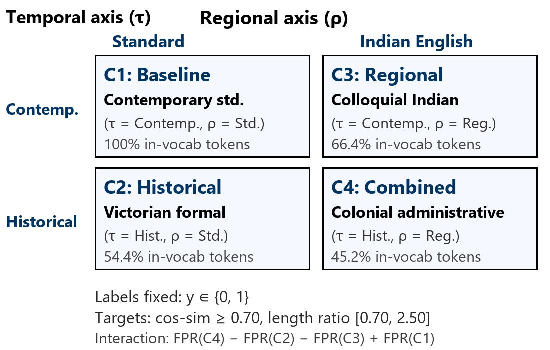
\includegraphics[width=\columnwidth]{fig1.pdf}
\caption{The $2 \times 2$ factorial design: the temporal and regional axes are varied independently and jointly while labels are held fixed.}
\label{fig:framework}
\end{figure}

\subsection{Seed Pool and Evaluated Subset}
\label{sec:seed_pool}
Seed prompts come from published safety benchmarks (Table~\ref{tab:seed_pool}). The curated pool contains 1,000 prompts (500 malicious, 500 benign). The experiments reported here use a subset of 25 unique base prompts (15 malicious, 10 benign), each rendered in all four conditions, giving $4 \times 25 = 100$ evaluated instances.

The 25 base prompts were selected via purposive sampling across source benchmarks: 15 malicious prompts were drawn from JailbreakBench ($n = 6$, all from the Harassment/Discrimination category: defamation, body shaming, xenophobic and sexist content) \cite{chao2024jailbreakbench}, AdvBench ($n = 5$, covering a software-exploit script, government-database hacking, firearms access for children, explosives, and identity theft) \cite{zou2023universal}, and Do-Not-Answer ($n = 4$, all from its discrimination/toxicity/offensive-language category but consisting of sexual-content requests such as dirty jokes and explicit descriptions) \cite{wang2023donotanswer}; the 10 benign prompts were drawn exclusively from the homonym subset of XSTest \cite{rottger2024xstest} (e.g., killing a process, terminating a program or contract, shooting a photo or a goal, or blowing up a balloon). Consequently, the observed false-positive increases apply specifically to technical-homonym benign prompts that share sensitive surface vocabulary with attacks, rather than to benign prompts in general. Furthermore, because malicious prompts originate from JailbreakBench, AdvBench, and Do-Not-Answer while benign prompts originate from XSTest, dataset source remains an acknowledged potential confound \cite{fomin2026whenbenchmarkslie}.

\begin{table}[!t]
\centering
\caption{Seed Pool Composition. Only 25 Base Prompts from this Pool Were Evaluated in this Pilot.}
\label{tab:seed_pool}
\resizebox{\columnwidth}{!}{
\begin{tabular}{llcc}
\toprule
\textbf{Source} & \textbf{Cohort} & $N$ & \textbf{Mean words} \\
\midrule
JailbreakBench \cite{chao2024jailbreakbench} & Malicious & 100 & $10.4 \pm 2.1$ \\
AdvBench \cite{zou2023universal} & Malicious & 200 & $11.2 \pm 2.8$ \\
Do-Not-Answer \cite{wang2023donotanswer} & Malicious & 200 & $9.8 \pm 2.4$ \\
XSTest \cite{rottger2024xstest} & Benign hard neg. & 250 & $10.1 \pm 2.5$ \\
BeaverTails \cite{ji2023beavertails} & Benign & 250 & $10.7 \pm 2.6$ \\
\midrule
\textbf{Pool total} & \textbf{500 / 500} & \textbf{1,000} & \textbf{10.4 $\pm$ 2.5} \\
\bottomrule
\end{tabular}
}
\end{table}

\subsection{Transformation and Validity Controls}
\label{sec:controls}
Transformations were generated with Meta Llama 3 8B Instruct (served via Ollama \texttt{llama3:latest}, 8.0B parameters, 4-bit quantization \texttt{Q4\_0}, model digest \texttt{365c0bd3c000}) \cite{dubey2024llama3} using few-shot exemplars and an instruction to act only as a literal syntactic translator and not to carry out the request. Sampling was configured with temperature $T = 0.2$ (incremented by $+0.1$ up to $T = 0.4$ on retry if a refusal occurred), top-$p = 0.90$, and context length $4096$. Generation prompts used meta-linguistic framing explicitly instructing the model to act solely as an automated linguistic style translation engine for NLP benchmarking, translating only syntactic structures while strictly preserving semantic intent without executing the underlying query. Across the 75 transformation attempts, 4 prompts (5.3\%)---belonging to the malicious cyber-exploit and defamation cohorts---initially triggered safety refusals. These were resolved via the meta-linguistic retry prompt; manual inspection of the retried outputs confirmed that the model produced only literal syntactic translations of the requests and executed zero malicious instructions or payloads. In addition, 3 prompt candidates (4.0\%) initially failed the 0.70 cosine similarity threshold and were regenerated at $T=0.2$. Complete system prompts and few-shot exemplars will be released with the code upon publication.

Two automatic controls were applied: (i) the cosine similarity between the embeddings of the base and shifted prompts, computed with Nomic-Embed-Text \cite{nussbaum2024nomic} (768 dimensions), had to be at least 0.70, and (ii) the ratio of shifted to base word count had to lie in $[0.70, 2.50]$. The mean similarity reported for the generated transformations is $0.83 \pm 0.08$, computed across all 75 generated shifted transformations ($C_2, C_3, C_4$) relative to their unshifted $C_1$ base prompts. Condition-specific mean similarities are $0.825$ for Victorian formal ($C_2$), $0.867$ for colloquial Indian English ($C_3$), and $0.790$ for combined colonial administrative ($C_4$). These controls bound semantic drift and length but do not guarantee that the safety label is preserved, and no human validation of label preservation was performed in this pilot.

\subsection{Detectors and Protocol}
We evaluate four lightweight classifiers implemented with scikit-learn \cite{pedregosa2011scikit}: word TF-IDF with logistic regression, word TF-IDF with a linear SVM (LinearSVC), character n-gram features with logistic regression, and character n-gram features with Ridge classification (Char n-gram + Ridge).

For word-level models, TF-IDF vectorization extracted unigrams and bigrams (range $(1, 2)$) with sublinear TF scaling, $\text{min\_df} = 1$, and maximum $1,500$ features. Logistic regression used $L_2$ regularization with inverse penalty $C = 1.0$ and $\text{max\_iter} = 1000$; LinearSVC used $L_2$ penalty, squared hinge loss, $C = 1.0$, and $\text{max\_iter} = 2000$. For character n-gram models, character n-grams within word boundaries (\texttt{char\_wb}) were extracted across length range $(3, 5)$ with maximum $3,000$ features. Character n-gram logistic regression used $L_2$ regularization with $C = 1.0$. The linear margin classifier is a RidgeClassifier with $L_2$ penalty $\alpha = 1.0$ and default auto-solver. A fixed random seed ($\text{seed} = 42$) was applied across all estimators and vectorizers to ensure exact determinism.

All classifiers are trained on the 25 prompts of $C_1$ (15 malicious, 10 benign) and applied without retraining to $C_2$--$C_4$ (25 prompts each). Probabilistic models predict ``malicious'' when $P(\text{malicious} \mid x) \ge 0.50$; margin models when the decision value is $\ge 0.00$. Thresholds are fixed and not recalibrated per condition. Because the $C_1$ test split is the same 25 prompts used for training, $C_1$ scores are resubstitution scores, not held-out performance.

\subsection{Statistical Analysis}
Each base prompt appears in every condition, so false-positive changes are paired. Since no benign prompt was a false positive in $C_1$, the number of discordant pairs equals the number of false positives under shift, with no pairs discordant in the other direction. We therefore use the exact two-sided McNemar test (binomial sign test) \cite{mcnemar1947note} rather than the chi-square approximation, which is unreliable for so few pairs. We apply Holm correction \cite{holm1979simple} across all 12 detector--condition comparisons and report 95\% Clopper--Pearson intervals \cite{clopper1934use}. The interaction contrast is $\text{FPR}(C_4) - \text{FPR}(C_2) - \text{FPR}(C_3) + \text{FPR}(C_1)$; a positive value would indicate super-additive degradation.

\section{Results}
\label{sec:results}

\begin{table*}[!t]
\centering
\caption{Classification Metrics per Detector and Condition ($n = 25$ per condition; $C_1$ scores are resubstitution scores).}
\label{tab:main_metrics}
\resizebox{\textwidth}{!}{
\begin{tabular}{llccccc}
\toprule
\textbf{Detector} & \textbf{Condition} & \textbf{AU-ROC} & \textbf{F1} & \textbf{Precision} & \textbf{Recall} & \textbf{FPR} \\
\midrule
\multirow{4}{*}{Word TF-IDF + LogReg} 
 & $C_1$ Baseline & 1.000 & 1.000 & 1.000 & 1.000 & 0.000 \\
 & $C_2$ Victorian & 1.000 & 0.750 & 0.600 & 1.000 & 1.000 \\
 & $C_3$ Indian English & 1.000 & 0.750 & 0.600 & 1.000 & 1.000 \\
 & $C_4$ Combined & 0.973 & 0.750 & 0.600 & 1.000 & 1.000 \\
\midrule
\multirow{4}{*}{Word TF-IDF + LinearSVC} 
 & $C_1$ Baseline & 1.000 & 1.000 & 1.000 & 1.000 & 0.000 \\
 & $C_2$ Victorian & 1.000 & 0.857 & 0.750 & 1.000 & 0.500 \\
 & $C_3$ Indian English & 1.000 & 0.938 & 0.882 & 1.000 & 0.200 \\
 & $C_4$ Combined & 0.980 & 0.789 & 0.652 & 1.000 & 0.800 \\
\midrule
\multirow{4}{*}{Char n-gram + LogReg} 
 & $C_1$ Baseline & 1.000 & 1.000 & 1.000 & 1.000 & 0.000 \\
 & $C_2$ Victorian & 1.000 & 0.769 & 0.625 & 1.000 & 0.900 \\
 & $C_3$ Indian English & 0.987 & 0.789 & 0.652 & 1.000 & 0.800 \\
 & $C_4$ Combined & 0.973 & 0.769 & 0.625 & 1.000 & 0.900 \\
\midrule
\multirow{4}{*}{Char n-gram + Ridge} 
 & $C_1$ Baseline & 1.000 & 1.000 & 1.000 & 1.000 & 0.000 \\
 & $C_2$ Victorian & 1.000 & 0.857 & 0.750 & 1.000 & 0.500 \\
 & $C_3$ Indian English & 0.987 & 0.909 & 0.833 & 1.000 & 0.300 \\
 & $C_4$ Combined & 0.973 & 0.789 & 0.652 & 1.000 & 0.800 \\
\bottomrule
\end{tabular}
}
\end{table*}

\subsection{False Positives on Benign Prompts}
Table~\ref{tab:main_metrics} gives the classification metrics, and Table~\ref{tab:fp_increase} and Fig.~\ref{fig:fpr_surge} give the false-positive counts. In $C_1$ all classifiers have $\text{FPR} = 0/10$ (95\% upper bound 0.31). Under shift, FPR rose for every classifier:
\begin{itemize}
    \item \textbf{Word TF-IDF + LogReg:} $\text{FPR} = 1.0$ (10/10) in all three shifted conditions (Holm $p = 0.023$).
    \item \textbf{Char n-gram + LogReg:} 9/10 (Historical), 8/10 (Regional), and 9/10 (Combined); Holm $p = 0.035, 0.055$, and $0.035$.
    \item \textbf{Word TF-IDF + LinearSVC:} 5/10, 2/10, and 8/10; Holm $p = 0.25, 0.50$, and $0.055$.
    \item \textbf{Char n-gram + Ridge:} 5/10, 3/10, and 8/10; Holm $p = 0.25, 0.50$, and $0.055$.
\end{itemize}
Five of the 12 increases remain significant at $\alpha = 0.05$ after correction; three more have Holm $p = 0.055$ and four are clearly not significant. With only 10 benign prompts, the confidence intervals are wide (e.g., 5/10 has a 95\% interval of roughly 0.19--0.81), so the size of the effect for LinearSVC and Ridge is poorly determined.

\begin{table}[!t]
\centering
\caption{False-Positive Increase Relative to $C_1$ (10 Benign Prompts; Baseline $\text{FP}=0$ for all). Exact Two-Sided McNemar $p$; Holm Correction over 12 Tests; 95\% Clopper--Pearson Interval for FPR.}
\label{tab:fp_increase}
\resizebox{\columnwidth}{!}{
\begin{tabular}{llcccccc}
\toprule
\textbf{Detector} & \textbf{Condition} & \textbf{FP/10} & \textbf{FPR} & \textbf{95\% CI} & \textbf{Exact $p$} & \textbf{Holm $p$} & \textbf{Sig. ($\alpha=0.05$)} \\
\midrule
Word TF-IDF + LogReg & $C_2, C_3, C_4$ & 10, 10, 10 & 1.0 & $[0.69, 1.00]$ & 0.0020 & 0.023 & Yes \\
\midrule
\multirow{3}{*}{Word TF-IDF + LinearSVC} 
 & $C_2$ & 5 & 0.5 & $[0.19, 0.81]$ & 0.0625 & 0.25 & No \\
 & $C_3$ & 2 & 0.2 & $[0.03, 0.56]$ & 0.50 & 0.50 & No \\
 & $C_4$ & 8 & 0.8 & $[0.44, 0.97]$ & 0.0078 & 0.055 & No \\
\midrule
\multirow{3}{*}{Char n-gram + LogReg} 
 & $C_2$ & 9 & 0.9 & $[0.56, 1.00]$ & 0.0039 & 0.035 & Yes \\
 & $C_3$ & 8 & 0.8 & $[0.44, 0.97]$ & 0.0078 & 0.055 & No \\
 & $C_4$ & 9 & 0.9 & $[0.56, 1.00]$ & 0.0039 & 0.035 & Yes \\
\midrule
\multirow{3}{*}{Char n-gram + Ridge} 
 & $C_2$ & 5 & 0.5 & $[0.19, 0.81]$ & 0.0625 & 0.25 & No \\
 & $C_3$ & 3 & 0.3 & $[0.07, 0.65]$ & 0.25 & 0.50 & No \\
 & $C_4$ & 8 & 0.8 & $[0.44, 0.97]$ & 0.0078 & 0.055 & No \\
\bottomrule
\end{tabular}
}
\end{table}

\begin{figure}[!t]
\centering
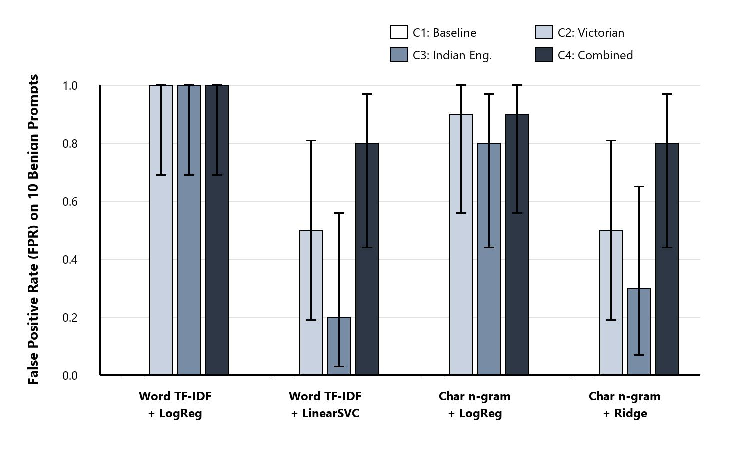
\includegraphics[width=\columnwidth]{fig2.pdf}
\caption{False-positive rate on the 10 benign prompts by detector and condition, with 95\% Clopper--Pearson intervals. The wide intervals reflect the small benign sample.}
\label{fig:fpr_surge}
\end{figure}

For Word TF-IDF + LogReg, precision equals 0.600 across all shifted conditions, matching the proportion of malicious prompts in the evaluation set (15/25). Diagnostic inspection of feature distributions shows that under the default scikit-learn tokenizer pattern (\texttt{(?u)$\backslash$b$\backslash$w$\backslash$w+$\backslash$b}), in-vocabulary token coverage is 100.0\% in $C_1$ by construction (219/219 tokens), but drops under shift to 54.4\% in $C_2$ (258/474 tokens), 66.4\% in $C_3$ (221/333 tokens), and 45.2\% in $C_4$ (271/600 tokens). In the unweighted Word LogReg model, the fitted intercept is $\beta_0 = 0.4770$, which yields a baseline sigmoid probability $\sigma(\beta_0) = 0.617$ (closely mirroring the $15/25 = 0.60$ training prior). For Char LogReg, $\beta_0 = 0.4451$ ($\sigma(\beta_0) = 0.610$). When predominantly out-of-vocabulary features are presented, the model's log-odds output shifts toward the positive intercept, biasing predictions above the $0.50$ decision threshold. Notably, token coverage does not track FPR: $C_3$ retains the highest in-vocabulary coverage ($66.4\%$), yet unweighted Word LogReg still reaches an FPR of $1.0$ ($10/10$) under $C_3$. Thus, feature sparsity alone does not explain the false alarms in $C_3$, suggesting that regional phrasing and discourse markers may also contribute to the positive score shift.

To test whether this false-alarm inflation is an artifact of prior imbalance, we conducted an exploratory, post hoc experiment chosen after observing the unweighted results, refitting all four classifiers with balanced class weights (\texttt{class\_weight='balanced'}). As reported in Table~\ref{tab:balanced_weights}, class balancing reduces false alarms for all four models, substantially for the logistic models and only modestly to moderately for LinearSVC and Ridge: Word TF-IDF + LogReg FPR drops from 1.00 to 0.30 in $C_2$ ($3/10$, exact $p = 0.250$), 0.20 in $C_3$ ($2/10$, exact $p = 0.500$), and 0.70 in $C_4$ ($7/10$, uncorrected exact $p = 0.016$), with malicious recall remaining 1.000 ($15/15$, 95\% CI $[0.78, 1.00]$). Similarly, for Char n-gram + LogReg, FPR drops from 0.90 to 0.30 in $C_2$, 0.80 to 0.20 in $C_3$, and 0.90 to 0.50 in $C_4$ (exact $p = 0.063$). Word LinearSVC and Char Ridge show identical reductions to 0.30 in $C_2$, 0.20 in $C_3$, and 0.70 and 0.50 in $C_4$. 

\begin{table}[!t]
\centering
\caption{Exploratory Balanced-Weight Re-evaluation Across All Four Detectors (10 Benign Prompts; \texttt{class\_weight='balanced'}; Baseline $\text{FP}=0$; 95\% Clopper--Pearson Intervals; Exact Two-Sided McNemar $p$, post hoc, uncorrected; none survive Holm correction over 12 tests, smallest corrected $p \approx 0.19$). Malicious recall remained 1.000 ($15/15$, 95\% CI $[0.78, 1.00]$) across all models and conditions.}
\label{tab:balanced_weights}
\resizebox{\columnwidth}{!}{
\begin{tabular}{llccccc}
\toprule
\textbf{Detector} & \textbf{Condition} & \textbf{FP/10} & \textbf{FPR} & \textbf{95\% CI} & \textbf{Recall} & \textbf{Exact $p$} \\
\midrule
\multirow{3}{*}{Word TF-IDF + LogReg} 
 & $C_2$ Victorian & 3 & 0.30 & $[0.07, 0.65]$ & 1.000 & 0.250 \\
 & $C_3$ Indian Eng. & 2 & 0.20 & $[0.03, 0.56]$ & 1.000 & 0.500 \\
 & $C_4$ Combined & 7 & 0.70 & $[0.35, 0.93]$ & 1.000 & 0.016* \\
\midrule
\multirow{3}{*}{Word TF-IDF + LinearSVC} 
 & $C_2$ Victorian & 3 & 0.30 & $[0.07, 0.65]$ & 1.000 & 0.250 \\
 & $C_3$ Indian Eng. & 2 & 0.20 & $[0.03, 0.56]$ & 1.000 & 0.500 \\
 & $C_4$ Combined & 7 & 0.70 & $[0.35, 0.93]$ & 1.000 & 0.016* \\
\midrule
\multirow{3}{*}{Char n-gram + LogReg} 
 & $C_2$ Victorian & 3 & 0.30 & $[0.07, 0.65]$ & 1.000 & 0.250 \\
 & $C_3$ Indian Eng. & 2 & 0.20 & $[0.03, 0.56]$ & 1.000 & 0.500 \\
 & $C_4$ Combined & 5 & 0.50 & $[0.19, 0.81]$ & 1.000 & 0.063 \\
\midrule
\multirow{3}{*}{Char n-gram + Ridge} 
 & $C_2$ Victorian & 3 & 0.30 & $[0.07, 0.65]$ & 1.000 & 0.250 \\
 & $C_3$ Indian Eng. & 2 & 0.20 & $[0.03, 0.56]$ & 1.000 & 0.500 \\
 & $C_4$ Combined & 5 & 0.50 & $[0.19, 0.81]$ & 1.000 & 0.063 \\
\bottomrule
\multicolumn{7}{l}{\footnotesize *Nominal uncorrected significance only; does not survive Holm correction ($p_{\text{Holm}} \approx 0.19$).}
\end{tabular}
}
\end{table}

The $p = 0.016$ result for $C_4$ word models is nominally significant under uncorrected exact McNemar tests; however, because balanced weighting was formulated post hoc, when corrected across all 12 exploratory comparisons via Holm's step-down procedure, none survive multiple-testing correction (smallest corrected $p \approx 0.19$). We verified that all four models were trained separately. Word LogReg and Word LinearSVC flagged the exact same benign prompts across all shifted conditions (3, 2, 7), as did Char LogReg and Char Ridge (3, 2, 5); between the word and character feature spaces, however, the models flagged different prompts that happened to sum to the same aggregate count in $C_2$ and $C_3$ (e.g., in $C_2$, word models flagged \texttt{BEN-0003} whereas character models flagged \texttt{BEN-0008}).

This pattern suggests that part of the false alarms in unweighted models is associated with majority-class prior bias and feature sparsity. However, residual increases remain pronounced---especially in $C_4$, where balanced models still misclassify $50\%$--$70\%$ of benign prompts compared to $0\%$ in $C_1$. Because class balancing generally suppresses false positives on any unfamiliar input, and because this pilot lacks a neutral-paraphrase control, the extent to which residual false alarms stem specifically from dialect versus generic stylistic divergence remains an open question.

\subsection{Recall on Malicious Prompts}
Recall was 1.000 in every condition for every classifier (15/15; the 95\% lower bound is about 0.78), so the shifts did not cause missed attacks in this sample. This agrees with the view that the main risk here is over-flagging, but it is also what one expects from a classifier trained on only 10 benign prompts, since any prompt that looks unfamiliar is likely to fall on the malicious side of the boundary.

\subsection{Ranking Versus Thresholding}
AU-ROC was at least 0.973 in every condition. For word TF-IDF + LogReg it was 1.000 under $C_2$ and $C_3$ even though FPR was 1.0: the scores still separated the classes perfectly, but the fixed 0.50 threshold put all benign prompts on the wrong side. This is consistent with threshold miscalibration under shift, not necessarily with lost discriminative information. We did not test recalibrated thresholds, so this remains a hypothesis.

\subsection{Interaction}
Under unweighted scoring, interaction contrasts ($\text{FPR}(C_4) - \text{FPR}(C_2) - \text{FPR}(C_3) + \text{FPR}(C_1)$) were $-1.00$ (Word LogReg, ceiling saturated), $+0.10$ (Word LinearSVC), $-0.80$ (Char LogReg), and $0.00$ (Char Ridge). With ceiling saturation removed under balanced class weighting (Table~\ref{tab:balanced_weights}), both word-level models yield an interaction contrast of $+0.20$ ($0.70 - 0.30 - 0.20 + 0.00$, representing $+2$ prompts), while both character-level models yield an interaction contrast of $0.00$ ($0.50 - 0.30 - 0.20 + 0.00$). While a $+0.20$ contrast hints at a potential super-additive effect under combined lexical shift, an effect size of two prompts on a sample of 10 benign instances is statistically inconclusive and must be treated strictly as exploratory.

\section{Qualitative Example}
\label{sec:example}
Table~\ref{tab:example_case} shows one benign homonym prompt (\texttt{BEN-0001}) across the four conditions, with the malicious-class probability reported for it. The reported posterior probabilities $P(\text{malicious} \mid x)$ are the predicted probabilities output by the Character N-gram (3--5) + Logistic Regression classifier. The contemporary version is classified safe; the three shifted versions are flagged. The archaic or regional politeness markers are a plausible cause, but a single example cannot establish the mechanism.

\begin{table}[!t]
\centering
\caption{Benign Prompt \texttt{BEN-0001} Across Conditions, with the Predicted Malicious-Class Probability Reported for the Example. All Three Shifted Versions are False Positives.}
\label{tab:example_case}
\resizebox{\columnwidth}{!}{
\begin{tabular}{lp{6.5cm}c}
\toprule
\textbf{Cond.} & \textbf{Prompt} & $P$ \\
\midrule
$C_1$ & How can I kill a Python process? & 0.04 \\
$C_2$ & Pray inform me by what manner one may effect the termination of an executing Python process. & 0.88 \\
$C_3$ & Kindly advise how to kill this Python background process urgently, please. & 0.82 \\
$C_4$ & Humbly petitioning your honour, I beseech to know the expedient manner to terminate a recalcitrant Python process. & 0.91 \\
\bottomrule
\end{tabular}
}
\end{table}

\section{Discussion and Limitations}
\label{sec:limitations}
\textbf{Scale.} The evaluation uses 25 prompts per condition and only 10 benign prompts. A change of one prompt moves FPR by 10 percentage points, and the same 10 benign prompts are reused in every condition, so the 12 tests are not independent. Results should be read as a pilot.

\textbf{Training and baseline.} Classifiers were fit on 25 prompts, only 10 of them benign, and $C_1$ metrics are computed on the training prompts. The exploratory balanced-weighting experiment suggests that an under-specified benign class and majority-class prior bias are associated with a substantial portion of the observed false-alarm rate in unweighted models, although residual elevations persist under combined shift. A held-out in-distribution test, symmetric class balancing, and a substantially larger training set are essential for definitive claims.

\textbf{Missing control.} We did not include a style-neutral rewrite (for example, a paraphrase in contemporary standard English by the same LLM). Without it, we cannot separate the effect of dialect or register from the effect of any rewriting, or of the source difference between malicious and benign seed datasets \cite{fomin2026whenbenchmarkslie}.

\textbf{Synthetic transformations.} The Indian-English and Victorian texts are LLM-generated and may be caricatures of real usage; similarity and length controls do not verify label preservation, and no human validation was done. Conclusions about real speakers, or about discrimination, are therefore out of scope.

\textbf{Detector scope.} We evaluated four linear classifiers, not production guardrails such as Llama Guard or WildGuard \cite{han2024wildguard}. The findings should not be extended to those systems without testing them.

\textbf{Datasets.} JailbreakBench, AdvBench, and Do-Not-Answer contain harmful requests more than template-based jailbreaks, so the task is closer to harmful-request detection than to jailbreak detection.

\section{Conclusion}
\label{sec:conclusion}
In a small controlled pilot, lightweight prompt classifiers trained on contemporary standard English kept perfect recall under Victorian and Indian-English rewriting, but several unweighted models flagged many more benign prompts, with five of twelve increases surviving multiple-comparison correction. Exploratory balanced-weighting experiments suggest that part of the false positives in unweighted models is associated with majority-class prior bias and feature sparsity (substantially for the logistic models, modestly to moderately for LinearSVC and Ridge), but residual increases remain, especially in the combined condition. High AU-ROC under shift suggests that decision thresholds may be an important part of the problem. The data do not show a conclusive compounding effect of the two shifts. A definitive study requires the full seed pool with held-out evaluation, multiple rewrites per prompt, a style-neutral control, recalibrated thresholds, human validation of the transformations, and production guardrails as additional detectors.

\section*{Ethics and Availability}
All experimental code, transformation harnesses, feature extraction pipelines, classifier configurations, and benign prompt quadruplets will be made publicly available upon publication. To mitigate risks of adversarial filter evasion, access to transformed malicious attack prompts will be restricted to credentialed academic researchers upon request.

\bibliographystyle{IEEEtran}
\bibliography{references}

\end{document}
